\chapter{Sphere collision}
\label{cha:spherecollision}

Spheres are the simplest of bounding shapes used in collision detection. This chapter presents tests for two versions of algorithms - naive $O(N^2)$ approach and with partitioned space. While simpler algorithm has far greater number of collision checks per frame, it allocates almost no memory per frame. More complex method will minimise number of checks, but additional structure and steps added may influence overall execution time in unexpected way.


\begin{figure}[h!]
  \caption{Example rendering of tested sphere collision system}
  \label{img:spheres}
  \centering
	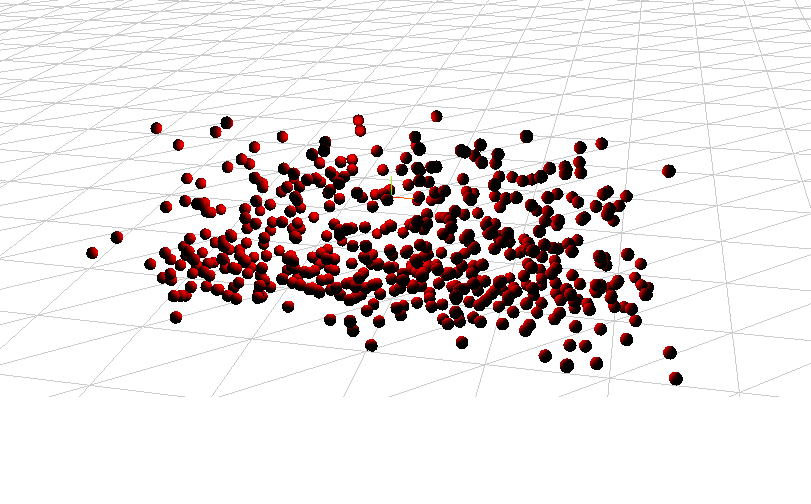
\includegraphics[width=16cm]{spheres/render.png}
\end{figure}

\section{Algorithm description}
\label{sec:spherealgorithmdescription}

Collision detection for spheres is a trivial task. If distance between two spheres is smaller than sum of their radiuses, spheres collide.

$\sqrt{(S_1.x - S_2.x)^2 + (S_1.y - S_2.y)^2 + (S_1.z - S_2.z)^2} < S_1.radius + S_2.radius$

While the equation is simple, with large number N of colliding objects complexity of this detection is $O(N^2)$. Methods of space partitioning are used to reduce number of checks. One used in this benchmark is Octree.
Base for algorithm is a tree-like structure of bounding boxes. Whenever a box contains more than one colliding object, it's divided into eight smaller boxes, by partitioning each edge by 2. When maximum tree depth is reached, multiple objects are stored in one box. One object may be referenced from multiple boxes, when it's size and position make them intersect. Each movement requires a check if object has already moved to one of neighbour boxes.

\begin{figure}[h!]
  \caption{Octree structure. Source: http://en.wikipedia.org/wiki/File:Octree2.svg/}
  \label{img:octree2}
  \centering
	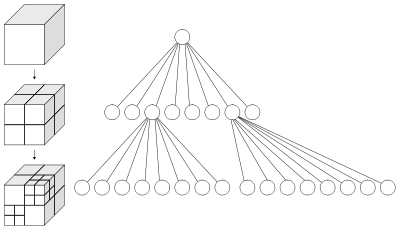
\includegraphics[width=10cm]{octree/octree2.png}
\end{figure} 

Having objects grouped in boxes reduces complexity of collision check. Since an object may collide only with objects in the same box, number of checks is much smaller. Overall complexity of Octree checks is $O(N log{N})$.
TODO: reference for complexity.

\begin{figure}[h!]
  \caption{Example of WebGL Octree debug rendering. Available online at http://pawlowski.it/octtree/}
  \label{img:octree}
  \centering
	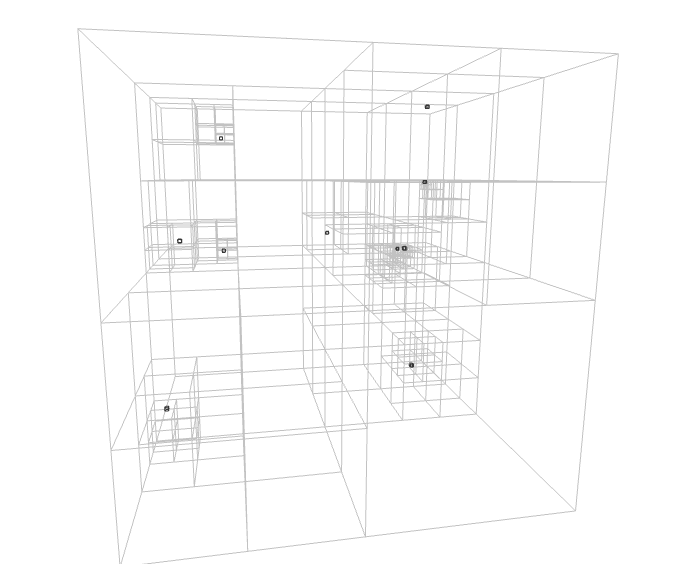
\includegraphics[width=10cm]{octree/octree.png}
\end{figure} 

When collision is detected, collision response is calculated. From rule of conservation of momentum:

\begin{center}
$m_1 * \vec{v_1} + m_2 * \vec{v_2} = m_1 * \vec{v'_1} + m_2 * \vec{v'_2}$
\end{center}

Meaning that change of both momentums is of equal value.
\begin{center}
$m_1*\vec{v'_1} =  m_1*\vec{v_1} - \Delta P$

$m_2*\vec{v'_2} =  m_2*\vec{v_2} + \Delta P$

$\vec{v'_1} =  \vec{v_1} - \frac{\Delta P}{m_1}$

$\vec{v'_2} =  \vec{v_2} + \frac{\Delta P}{m_2}$
\end{center}

To simplify response rotation and deformation of spheres are ignored. This does not affect performance analysis, since operations performed all tests is done in the same way.

Let
\begin{center}
$P = |\Delta P|$

$N = \hat{pos_1 - pos_2}$
\end{center}

Since transference of momentum occurs only along single point of contact:
\begin{center}
$ \Delta P = P * \hat{\vec{N}}$

$\vec{v'_1} =  \vec{v_1} - \frac{P}{m_1} * \vec{N}$

$\vec{v'_2} =  \vec{v_2} + \frac{P}{m_2} * \vec{N}$
\end{center}

Lets split each velocity into two scalars, perpendicular and parallel value of velocity vector, and introduce $\vec{Q}$, similar to $\vec{N}$, a perpendicular normalised vector lining along exchanged momentum.

 \begin{center}
$\vec{v_1} =  a_1 * \vec{N} + b_1 * \vec{Q}$

$\vec{v_2} =  a_2 * \vec{N} + b_2 * \vec{Q}$

$\vec{v'_1} =  a'_1 * \vec{N} + b'_1 * \vec{Q}$

$\vec{v'_2} =  a'_2 * \vec{N} + b'_2 * \vec{Q}$
\end{center}

\begin{figure}[h!]
  \caption{Illustration for collision response}
  \label{img:spheresbounce}
  \centering
	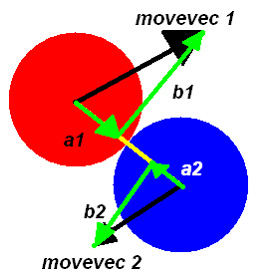
\includegraphics[width=8cm]{spheres/bounce.jpg}
\end{figure} 

Deriving from previous equations:

 \begin{center}
$a_1' =  a_1 - \frac{P}{m_1}$

$b_1' = b_1$

$a_2' =  a_2 + \frac{P}{m_2}$

$b_2' = b_2$
\end{center}

Now lets use rule of conservation of energy to solve P:

 \begin{center}
$\frac{m_1}{2} * ||\vec{v_1}||^2 + \frac{m_2}{2} * ||\vec{v_2}||^2 = \frac{m_1}{2} * ||\vec{v'_1}||^2 + \frac{m_2}{2} * ||\vec{v'_2}||^2$

$\frac{m_1}{2} * ({a_1}^2 + {b_1}^2) + \frac{m_2}{2} * ({a_2}^2 + {b_2}^2) = \frac{m_1}{2} * ({a'_1}^2 + {b'_1}^2) + \frac{m_2}{2} * ({a'_2}^2 + {b'_2}^2)2$

$P = \frac{2*m_1*m_2*(a_1-a_2)}{m_1+m_2}$
\end{center}

and finally, using result from conservation of momentum:

 \begin{center}
$\vec{v'_1} =  \vec{v_1} - \frac{2*(a_1-a_2)}{m_1+m_2} * m_2 * \vec{N}$

$\vec{v'_2} =  \vec{v_2} + \frac{2*(a_1-a_2)}{m_1+m_2} * m_1 * \vec{N}$
\end{center}

From this result, using only dot product of velocity vectors and normalised vector $pos_1 - pos_2$ correct response to collision is calculated. In tested scenarios mass of all spheres is equal since it doesn't affect complexity of calculations and produces less randomised results.


\section{{$O(N^2)$} approach}
\label{sec:sphereinitial}

Naive approach for collision detection proves to by easy to implement in JavaScript. Since almost no memory is allocated in each frame, no garbage collection issues appear. All methods are well defined and work mostly on floats. This results in highly optimised binary code produced by compiler, as shown on \ref{img:spheres1profile}.

\begin{figure}[h!]
  \caption{Chart of time used in optimised version of JavaScript}
  \label{img:spheres1profile}
  \centering
	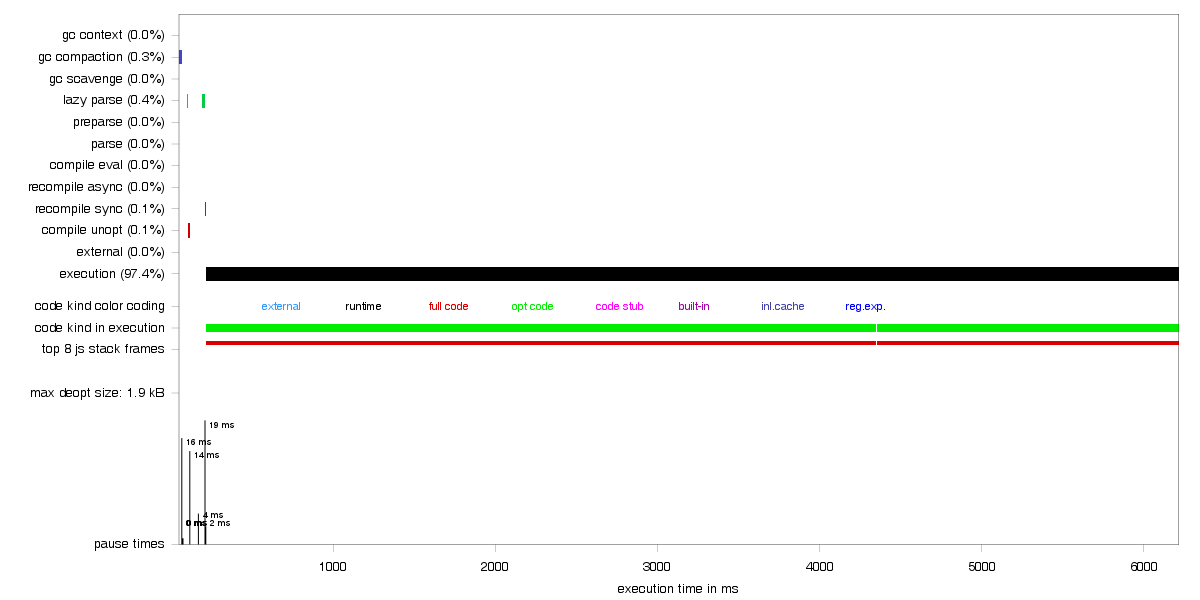
\includegraphics[width=16cm]{spheres/spheres1-profile.png}
\end{figure} 

Multiple tests with N=1000 and different number of frames rendered show, that for simple mathematical task performance of JavaScript is very close to this of C++. On average, JavaScript version of benchmark runs 15\% longer than C++ one.

\begin{figure}[h!]
  \caption{Comparison of total execution time. N = 1000, varying number of frames.}
  \label{img:spheres1-time-total}
  \centering
	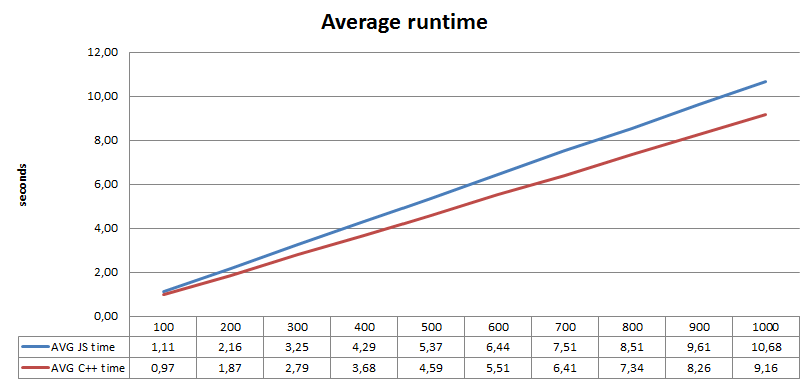
\includegraphics[width=16cm]{spheres/time-total.png}
\end{figure} 
\begin{figure}[h!]
  \caption{Comparison of execution time per frame. N = 1000, varying number of frames.}
  \label{img:spheres1-time-per-frame}
  \centering
	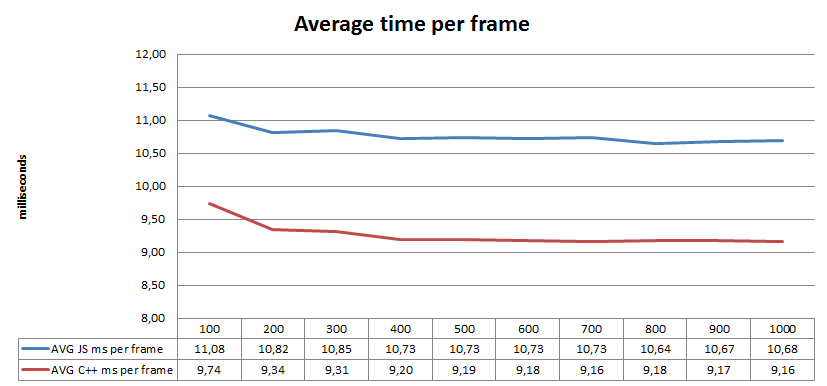
\includegraphics[width=16cm]{spheres/time-per-frame.png}
\end{figure}

\section{Octree-partitioned space}
\label{sec:sphereoctree}

\begin{figure}[h!]
  \caption{Octree partitioned sphere collision system}
  \label{img:spheres}
  \centering
	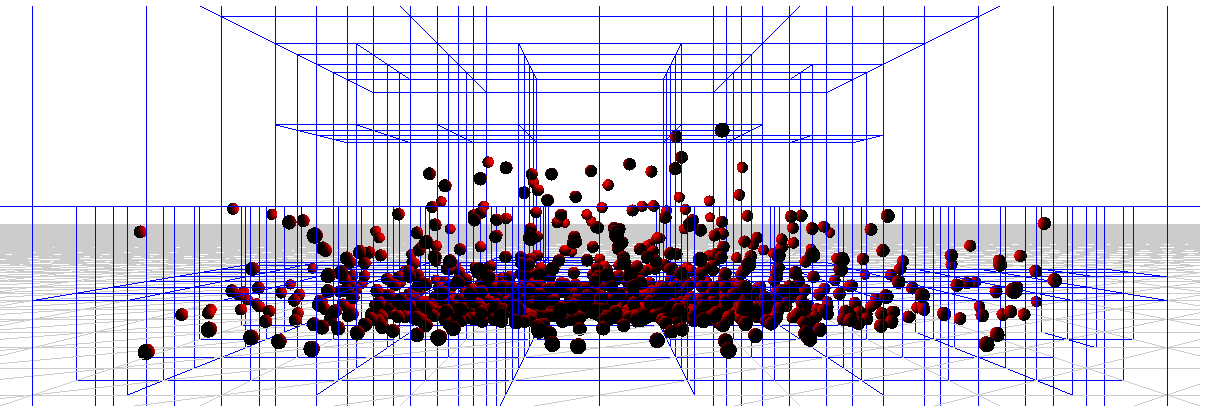
\includegraphics[width=16cm]{spheres/render2.png}
\end{figure}

Tests with Octree partitioning were executed with N=1000 spheres and T=1000 frames. Varying value is maximum depth of Octree, ranging from 1 to 10. 
Changing maximum depth reduces number of collision checks between spheres, as shown on \ref{img:octree-collisions}.

\begin{figure}[h!]
  \caption{Number of collisions in Octree}
  \label{img:octree-collisions}
  \centering
	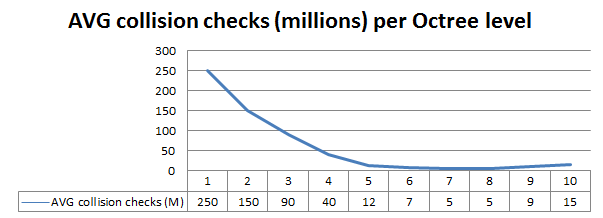
\includegraphics[width=16cm]{spheres/octree-collisions.png}
\end{figure}

For low values overall complexity of checks doesn't change significantly, since most of spheres are in one or few bounding cubes and no checks are skipped. Additional operations related to Octree are actually making this solution slower than $O(n^2)$ approach. For depth values in optimal zone, number of collision is reduced by factor of at least 10, while keeping Octree overhead reasonable. Interesting thing happens when maximum level of Octree is very high and edge of smallest Octree cube approaches size of spheres. Number of transitions between partitioning cubes, related memory allocation and cleanups actually make this approach much slower, as shown on \ref{img:octree-time}. Moreover, some spheres are references in more than one cube, raising again number of collision checks.

\begin{figure}[h!]
  \caption{Run times in Octree system}
  \label{img:octree-time}
  \centering
	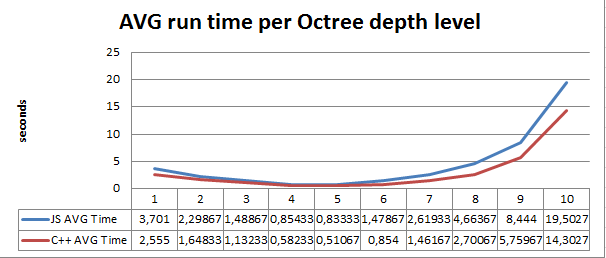
\includegraphics[width=16cm]{spheres/octree-time.png}
\end{figure}

It's clearly visible that number of collision checks and run time is correlated  only up to certain point. For deep Octrees number of checks doesn't improve further, but overall run time is getting longer. Performance of JavaScript in relation to C++ varies between 30\% to 80\% overhead. In comparison with $O(n^2)$ approach, optimal Octree in JavaScript runs over 92\% faster and C++ over 94\% faster. 
